\documentclass[8pt]{beamer}

%\beamertemplateshadingbackground{gray!0}{gray!50}
%\usepackage{beamerthemeshadow}
%\usetheme{Warsaw}
%\usetheme{Madrid}
%\setbeamercolor{background canvas}{bg=gray!10}
%\usepackage{beamerthemeclassic}
%
\usepackage{etex}
\usepackage[framesassubsections]{beamerprosper}
\usepackage{pstricks}
\usepackage{amsmath,amssymb,bbm,manfnt}
\usepackage{colortbl}
\usepackage[latin1]{inputenc}
\usepackage[T1]{fontenc} 
\usepackage{graphicx,psfrag}
\usepackage[english]{babel}
\usepackage{epsfig}
\usepackage{subfigure}
\usepackage{tikz}

%\usepackage{times}





\newcommand{\dps}{\displaystyle   }
\newcommand{\uu}[1]  {{{\boldsymbol #1}} }
\newcommand{\W}{\mathcal W}

\DeclareMathOperator*{\tendsto}{\longrightarrow}

\def\N{\mathbb{N}}
\def\R{\mathbb{R}}
\def\T{\mathbb{T}}
\def\Z{\mathbb{Z}}
\def\C{\mathbb{C}}

\def\E{\mathbb{E}} %esp\'erance
\def\P{\mathbb{P}} %probabilit\'e, \'el\'ements finis
\def\tr{\mathrm{tr}} %trace d'une matrice
\def\Var{\mathrm{Var}} %variance d'une variable al\'eatoire
\def\Vect{\mathrm{Vect}} %espace vectoriel engendr\'e par ...
\def\I{\mbox{Id}} % l'identité
\def\erf{\mbox{erf}} % fonction erreur

\definecolor{toto}{rgb}{0.2,0.2,0.7}

\def\div{{\rm div \;}}

\def\dt{\Delta t}
\def\sdt{\sqrt{\Delta t}}

\def\PP{\uu{P}}
\def\XX{\uu{X}}
\def\QQ{\uu{Q}}
\def\YY{\uu{Y}}
\def\ZZ{\uu{Z}}
\def\WW{\uu{W}}
\def\xx{\uu{x}}
\def\pp{\uu{p}}
\def\zz{\uu{z}}

\def\Var{\mathrm{Var}} %variance d'une variable al{\'e}atoire
\def\Covar{\mathrm{Covar}}
\def\Ker{\mathrm{Ker}}

\newcommand{\LJ}{{\rm LJ}_7^{{\rm 2D}}}
\newcommand{\tol}{{\rm TOL}}
\newcommand{\mean}[1]{\left\langle#1\right\rangle}
\newcommand{\corr}{\mathrm{corr}}
\newcommand{\prob}{\mathbb{P}}


\newcommand{\executeiffilenewer}[3]{%
  \ifnum\pdfstrcmp{\pdffilemoddate{#1}}%
                  {\pdffilemoddate{#2}}>0%
                  {\immediate\write18{#3}}\fi%
}
\newcommand{\includesvg}[1]{%
  \executeiffilenewer{#1.svg}{#1.pdf}%
                     {inkscape -z -D --file=#1.svg % 
                       --export-pdf=#1.pdf --export-latex}%
                     \input{#1.tex}%
}




% pour avoir le texte caché en gris
% \beamertemplatetransparentcovereddynamic

\title{Reliability of an option estimator on flight tickets}


\begin{document}

\frame{\titlepage}
%%%%%%%%%%%%%%%%%%%%%%%%%%%%%%%%%%%%%%%%%%%%%%%%%%%%%%%
\section{The aim of the estimator}
\subsection{The settings} 
\frame{
  The customer enters a set of criteria for its flight. In this work,
  only the following are considered
  \begin{itemize}
  \item the route (= (Paris - NYC,  2014-07-24, 2014-08-10)) 
  \item the start time $t_0$ (for the option),
  \item the demanded price $p_d$ (for the option),
  \item the expiry time $T$ at the option expires (for the option). 
  \end{itemize}
  We denote by $p(t,t_0,{\rm route})$ the flight price given by the
  travel agent at time $t\geq t_0$ for the route demanded. The option
  consists in hoping that there exists a time $t^*\in [ t_0, t_0+T]$
  such that
  $$
  p_d\geq p(t^*,t_0,{\rm route}).
  $$
  In that case, the option is terminated and the customer pays its
  tickets at the demanded price $p_d$. Else he doesn't travel!
}

\subsection{The goal of the estimator} 
\frame{ 
  \begin{itemize}
  \item When $(t_0,T,p_d)$ and the route are given, \textit{OPTION
    WAY} evaluates the possibility to terminate the option before time
    $t_0+T$ by returning a percentage
    $$
    \alpha(t_0,T, p_d, {\rm route})\in [0,1].
    $$

  \item \textbf{We will test if this alpha is sharp using the past
    prices for several routes. }\\
  \item We first need an indicator to test $\alpha$.
  \end{itemize}
}

\subsection{Examples of data} 
\frame{ 
  Paris-Rome, one week travel. Departure on saturday.
  \vspace{-0.4cm}
  \begin{center}
    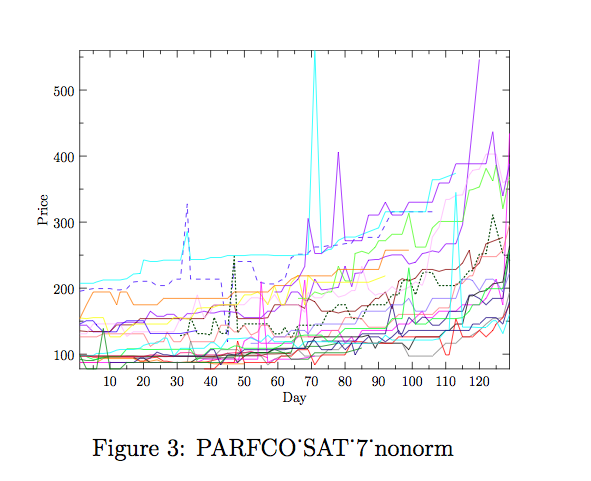
\includegraphics[width=7.cm]{picture1.png}
  \end{center}
  \vspace{-0.4cm}
}
\frame{ 
  Paris-La R\'eunion, one week travel. Departure on saturday.
  \vspace{-0.4cm}
  \begin{center}
    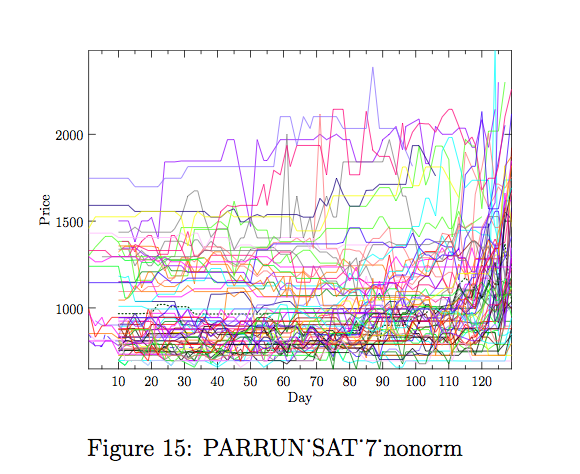
\includegraphics[width=7.cm]{picture2.png}
  \end{center}
  \vspace{-0.4cm}
}

\section{The test}
\subsection{Explanation of the test}
\frame{
  \textbf{Explanation:} we want to test the prediction of the
  relevance of the option given by OPTION WAY. \\
  Example: 
  \begin{itemize} 
  \item My travel lasts $20$ days and the departure in on Monday in
    two months.
  \item I demand a price $p_d$ for this specific flight.  
  \end{itemize}
  I enter information on the OPTION WAY website and I demand a one
  month option (one month = time limit) at price $p_d$. \\
  \begin{figure}
    \begin{center}
      \begin{tikzpicture}
        \tikzstyle{vertex}=[draw,circle,fill=blue,minimum size=6pt,inner sep=0pt]

        \draw[->] (0,0)--(8,0);


        \draw (0,0) node[vertex,label=below:{$0={\rm actual \ time}$}] (v) {};
        \draw (3.5,0) node[vertex,label=below:{$1={\rm option \ time \ limit}$}] (v) {};
        \draw (7,0) node[vertex,label=below:{$2={\rm departure }$}] (v) {};
      \end{tikzpicture}
      \caption{Times}
      \label{fig:contour}
    \end{center}
  \end{figure}
} \frame{
  $\to$ The OPTION WAY website returns a percentage $\red \alpha$ for
  the relevance of my option : what is the "probability" to find the
  flight ticket at price $p_d$ before this time limit ? It is $\red
  \alpha$. \\
  \textbf{Our question : is $\red \alpha$ a good estimator ?}
  We design these simple tests :
  \begin{enumerate}
  \item sample a collection of $\alpha(t_0,T,p_d, {\rm route})$ for
    several cases $(t_0,T,p_d, {\rm route})$ \textbf{in the past}.
  \item We define $V$ by $V(t_0,T,p_d,{\rm route}):=1$ if there exists
    a time $t^*\in [t_0,t_0+T]$, such that $p(t^*,t_0,{\rm route})\leq
    p_d$ (the option would have been realised).  Else
    $V(t_0,T,p_d,{\rm route}):=0$.
  \end{enumerate}
  $$\boxed{Test_1:=V-\alpha} \in [-1,1] $$
  $$\boxed{Test_2:=1-\vert Test_1\vert}\in [0,1]$$
}

\subsection{Remarks on the test}
\frame{
  Remarks on the test.
  \begin{itemize}
  \item if $Test_1:=V-\alpha \in [-1,1]$ is positive, $\alpha$ is
    pessimistic. If it is negative, $\alpha$ is optimistic.
  \item $Test_2:=1-\vert Test_1\vert \in [0,1]$ is the distance to the
    truth. The more it is closed to $1$, the better is the prediction
    $\alpha$ given by OPTION WAY.
  \end{itemize}
  With these $Test_1$ and $Test_2$ we can build some graphic
  representations to be able to compare $\alpha$ with the truth$V$. \\

}
\subsection{Expression of $\alpha$}
\frame{
  Expression of $\alpha$ chosen by OPTION WAY
  $$
  \alpha(t_0,T,p_d)=1/(1+\frac{4500p(t_0)}{10,5\times T}e^{-11\frac{p_d}{p(t_0)}}).
  $$
  $\to$ It is independent of the route, the past prices...\\
  This has the shape of a sigmoid ($f(x)=1/(1+e^{-x})$)
  \hspace{0.4cm}
  \begin{center}
    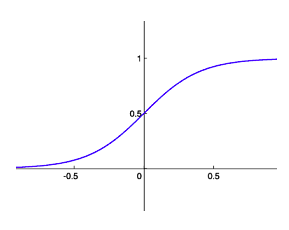
\includegraphics[width=4.cm]{sigmoid.png}
  \end{center}
  \vspace{-0.4cm}
}


\section{Results}
\subsection{First test}
\frame{
  First test, explanations.
  $$
  Test_2(t_0,T,p_d,{\rm route})=1-\vert (V-\alpha) (t_0,T,p_d,{\rm route})\vert.
  $$
  We fix the route and take the median of $T$ and $p_d$. \\
  This leads to a function of $t_0$ given the route:
  $$
  t_0\mapsto {\rm Median}_{T,p_d} [Test_2(t_0,T,p_d,{\rm route})]:= {\rm Score}(t_0,{\rm route}).
  $$
}
\frame{
  Results (1):
  \hspace{0.4cm}
  \begin{center}
    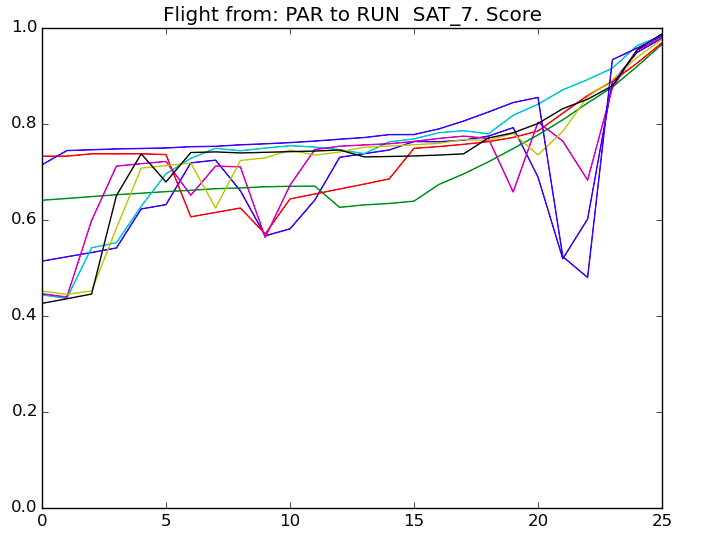
\includegraphics[width=7.cm]{res1.png}
  \end{center}
  \vspace{-0.4cm}
}
\frame{
  Results (2):
  \hspace{0.4cm}
  \begin{center}
    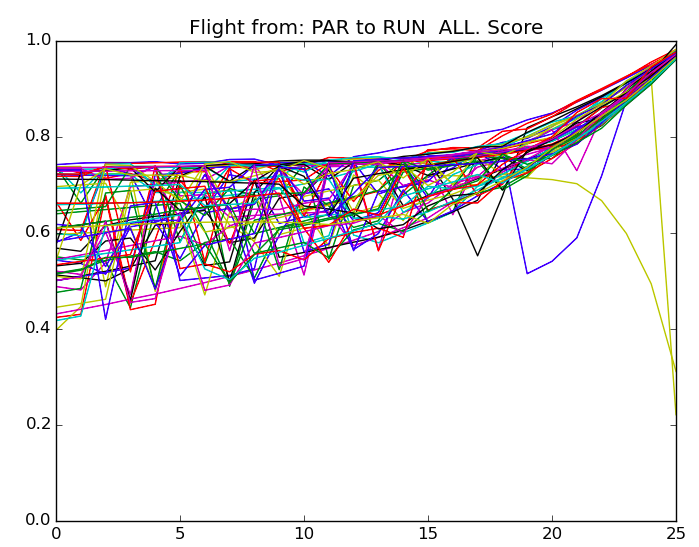
\includegraphics[width=7.cm]{res2.png}
  \end{center}
  \vspace{-0.4cm}
}
\frame{
  Results (3):
  \hspace{0.4cm}
  \begin{center}
    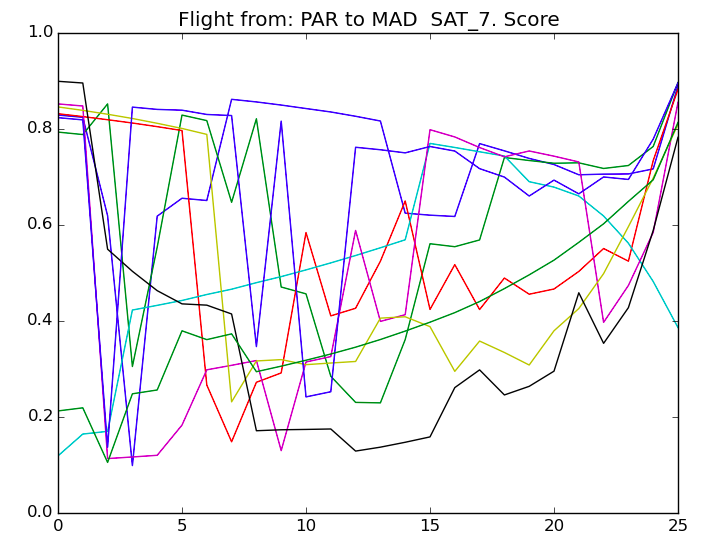
\includegraphics[width=7.cm]{res3.png}
  \end{center}
  \vspace{-0.4cm}
}
\subsection{Second test}
\frame{
  Second test, explanations.\\
  \begin{itemize}

  \item In the route, we fix the destination and the duration of the
    trip but not the departure time.  We fix $t_0$. We look at the
    matrix
    $$
    M_1: \ (T,p_d) \mapsto \sum \limits_{ {\rm departure \ day} } V(t_0, T, p_d, {\rm route}) / \sum \limits_{ {\rm departure \ day} } 1.
    $$
  \item and aslo
    $$
    M_2: \ (T,p_d) \mapsto \sum \limits_{ {\rm departure \ day} } [V-\alpha](t_0, T, p_d, {\rm route}) / \sum \limits_{ {\rm departure \ day} } 1.
    $$
 \end{itemize}
}

\frame{
  Results (1): $M_1$ for $t_0=20$ (normalised). The flight is
  Paris-Madrid, Monday 123 days.
  \hspace{0.4cm}
  \begin{center}
    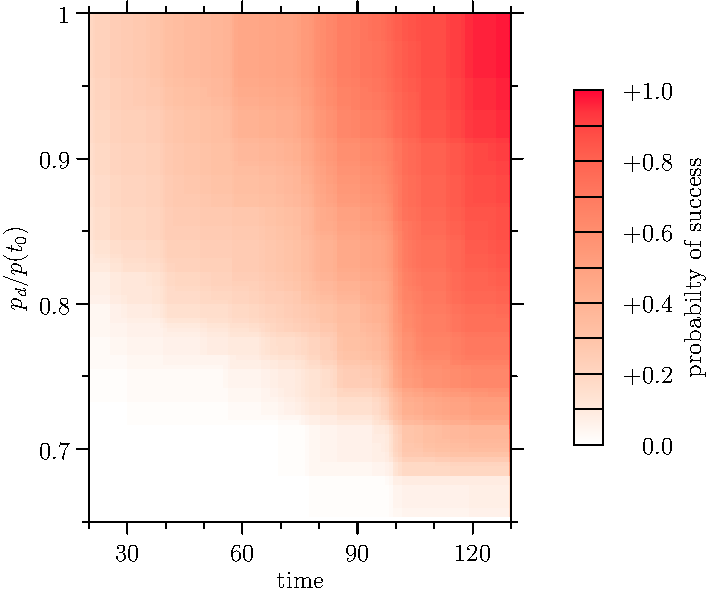
\includegraphics[width=8.cm]{res4.pdf}
  \end{center}
  \vspace{-0.4cm}
}

\frame{
  Results (2): $M_2$ for $t_0=20$ (normalised). The flight is
  Paris-Madrid, Monday 123 days.
  \hspace{0.4cm}
  \begin{center}
    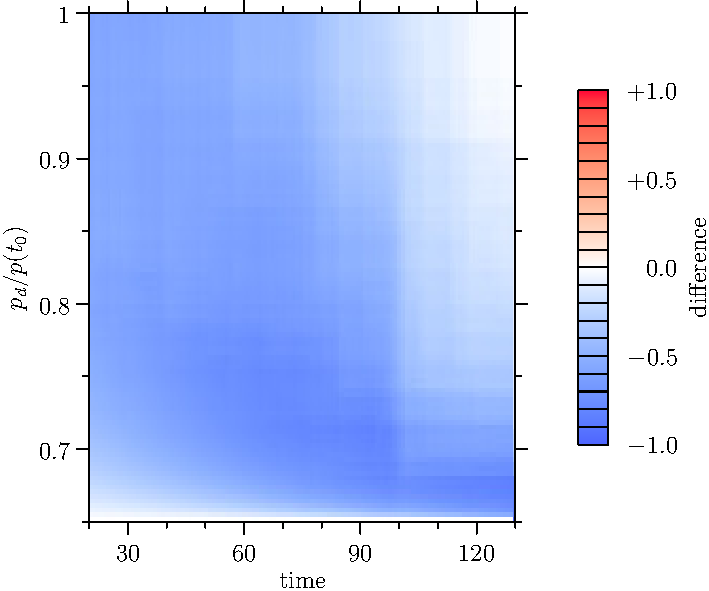
\includegraphics[width=8.cm]{res5.pdf}
  \end{center}
  \vspace{-0.4cm}
}

\frame{
  The last test. We look at the error:
  $$
  \mathcal E(t_0):=
  \Vert \overline V \Vert_{1, T\in [t_0,30], p_d\in [0,65\times p(t_0), p(t_0)]},
  $$
  where $\overline  V$ is  the mean over all the routes in the data.
}

\frame{
  Results (3):
  \hspace{0.4cm}
  \begin{center}
    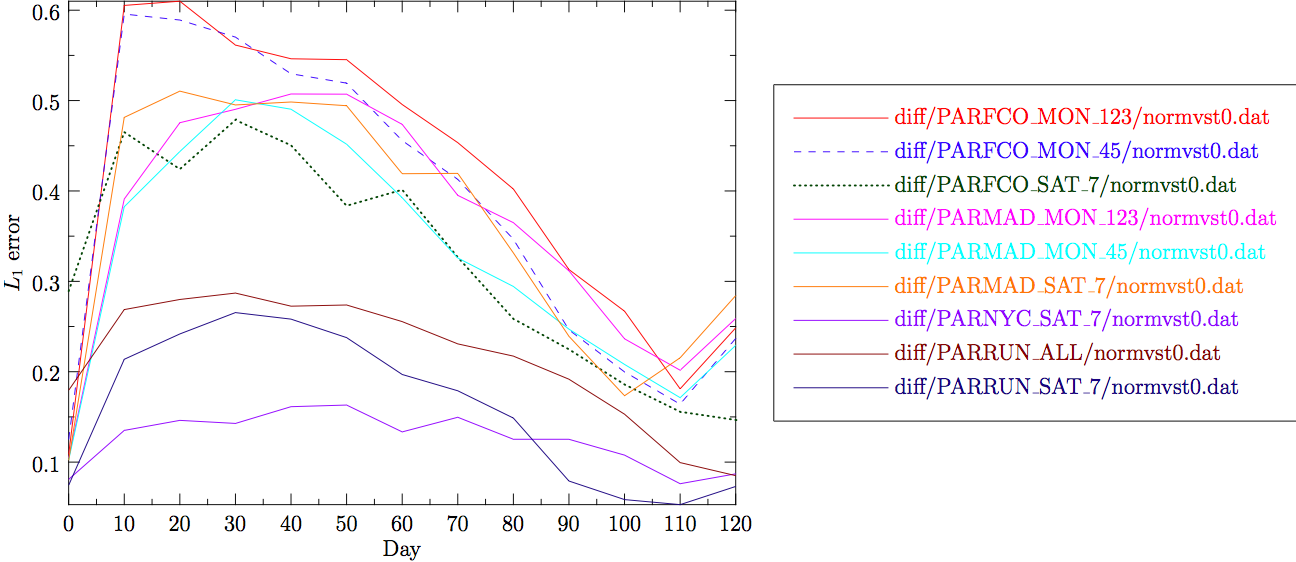
\includegraphics[width=10.cm]{res6.png}
  \end{center}
  \vspace{-0.4cm}
}

%% FIXME: Put tsuff here


 \frame{
 \frametitle{Calibration of the model }
 \begin{itemize} 
 \item Quadratic cost between the model and the observed data for a given rout $t_0$ 
 $$ J_{t_0} (a,b) = \dfrac{1}{2} \sum_{T} \sum_{P_d} \left( \alpha(a,b,T,P_d,p(t_0)) - V(T,P_d,p(t_0)) \right)^2 $$
 
 \item For every rout $t_0 \in (0,t_{max}]$, we would like to minimize the cost $ argmin_{(a,b) \in \R^*_+}   J_{t_0} (a,b) $ using a gradient based algorithm such as BFGS.  
%FIXME: argmin
 
 \end{itemize}


\begin{columns}
\begin{column}{6cm}
\begin{figure}
\centering
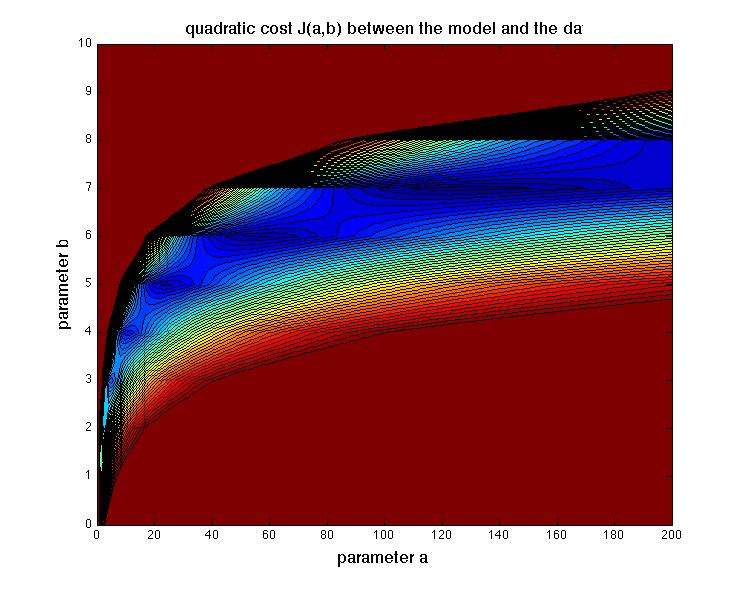
\includegraphics[width=6cm]{Cost.jpg}
\caption{$J$ in the region $(a,b) \in [0,200]\times[0,10]$}
\end{figure}
\end{column}



\begin{column}{6cm}
\begin{figure}
\centering
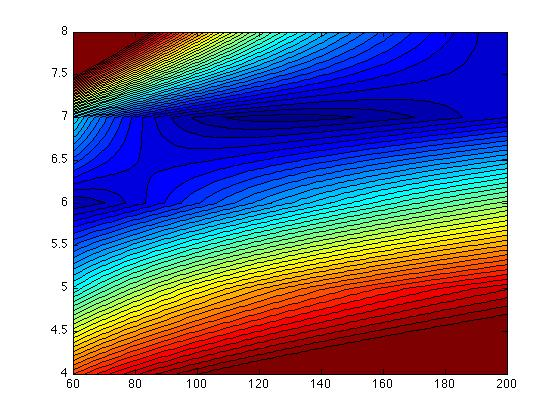
\includegraphics[width=6cm]{zoom_cost.jpg}
\caption{Zoom of $J$ over a and b}
\end{figure}
\end{column}
\end{columns}
 }
 
 
 
 
 \frame{
\frametitle{ A few examples of optimal parameters}
 \begin{figure}[h!]
 \centering
$$
\begin{array}{c|c|c|c|c|}
t_0 = 0 & 1 flight & 5 flights  & 10 flights & 50 flights \\
 \hline
a^*   			&- 	&192				&180		&182 \\
b^*			&- 	&11				&40		&39,5 \\
J(428,11) 	&- 	&2\times 10^{4}		&5\times 10^{4}		&2,6\times 10^{5}	 \\
J(a^*,b^*) 	&- 	&1,7\times 10^4	&1,8\times 10^{3}		&1,8\times 10^{3} \\
\| \nabla J(a^*,b^*) \|	&-	&10^{-2}		&10^{-3}		&10^{-3} \\
\end{array}
$$
\end{figure}



 \begin{figure}[h!]
 \centering
$$
\begin{array}{c|c|c|c|c|}
t_0 = 50 & 1 flight & 5 flights  & 10 flights & 50 flights \\
 \hline
a^*   					&140					&140					&140					&140 \\
b^*					&40 					&39					&40					&42 \\
J(428,11) 			&7\times  10^{4}	 	&4\times 10^{4}			&3,9\times 10^{4}		&3\times 10^{5}	 \\
J(a^*,b^*) 			&  1,3\times 10^4   		&1,3\times 10^3		&1,8\times 10^{3}		&1,9\times 10^{3} \\
\| \nabla J(a^*,b^*) \|	& 10^{-3}				&10^{-4}				&10^{-4}				&10^{-3} \\
\end{array}
$$
\end{figure}
}


 \frame{
   \frametitle{Possible improvement of the model}

   $$\beta(p_d, p(t_0), p_{min}, T) =  \dfrac{1}{1+ exp(-(\textcolor{blue}{S}-S_0)) + \dfrac{\textcolor{magenta}{d}}{T} +  \dfrac{\textcolor{magenta}{e} \times p_{min}}{max( p(t_0)-p_{min} , 10^{-14})}}$$


   \begin{itemize}
   \item The score S is defined by $\textcolor{blue}{S = \textcolor{magenta}{a} \dfrac{p_d}{p(t_0)} + \textcolor{magenta}{b} (1-  \dfrac{p_{min}}{p(t_0)} ) + \textcolor{magenta}{c} \dfrac{T}{T_f}} $
   \item $\dfrac{\textcolor{magenta}{c}}{T} $ : penalisation term of short times . 
   \item $ \dfrac{\textcolor{magenta}{d} \times p_{min}}{max( p(t_0)-p_{min} , 10^{-14})}$ : penalisation term of low prices. 
   \item $S_0$ : constant. 
   \end{itemize}

 }


\frame{
  \frametitle{comparaison of the models for the flight PARIS-NEW YORK }

  Form top to bottom and from left to right : the model $\alpha$ , the model $\beta$ with an exact estimation of $p_{min}$, $\beta$ with an over estimation of $p_{min}$and $\beta$ with an under estimation of $p_{min}$

  \begin{columns}
    \begin{column}{5cm}
      \begin{figure}
        \centering
        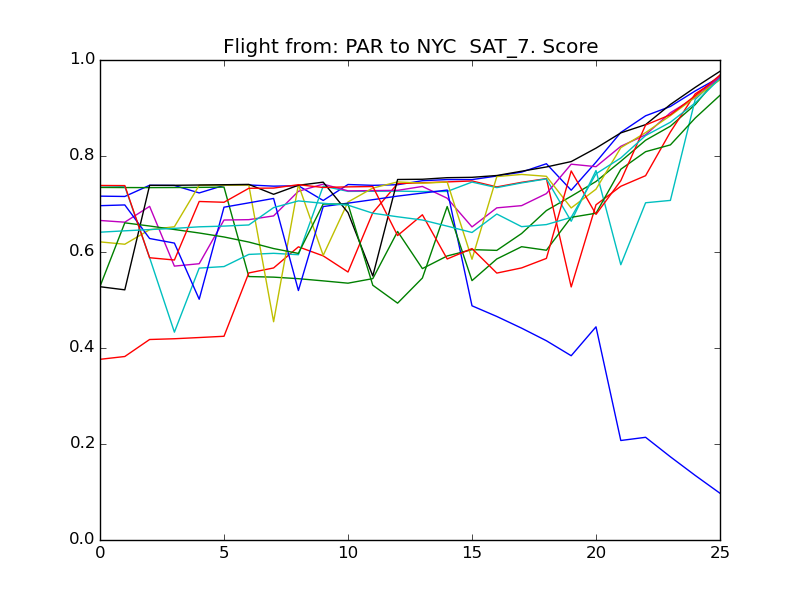
\includegraphics[width=5cm]{../ScoreImg/ScorePARNYC_SAT_7.png}
        %\caption{ the model $\alpha$ }
      \end{figure}

      \vspace{-0.8cm}
      \begin{figure}
        \centering
        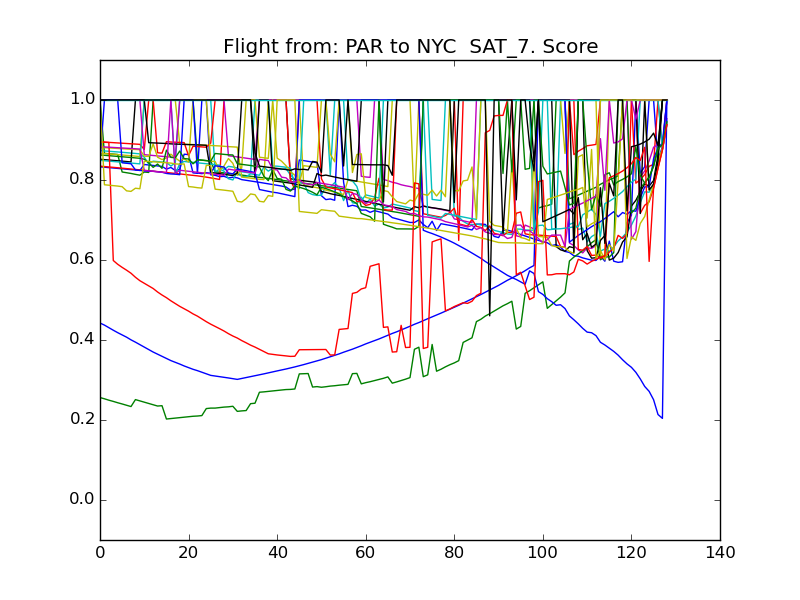
\includegraphics[width=5cm]{../ScorePRECISE/ScorePARNYC_SAT_7.png}
        %\caption{ the model $\beta$ with an exact estimation of $p_{min}$}
      \end{figure}
    \end{column}

    \begin{column}{5cm}
      \begin{figure}
        \centering
        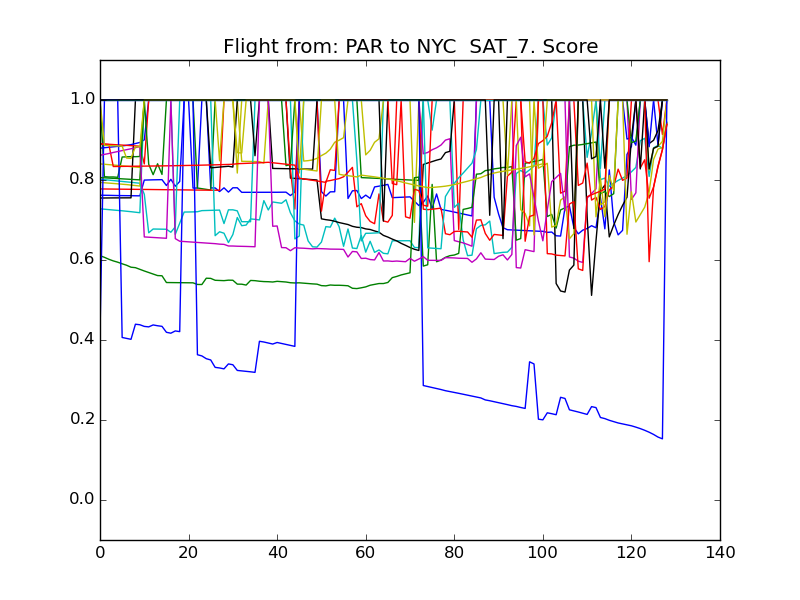
\includegraphics[width=5cm]{../ScoreOVERESTIMATE/ScorePARNYC_SAT_7.png}
        %\caption{ the model $\beta$ with an over estimation of $p_{min}$}
      \end{figure}
      \vspace{-0.8cm}
      \begin{figure}
        \centering
        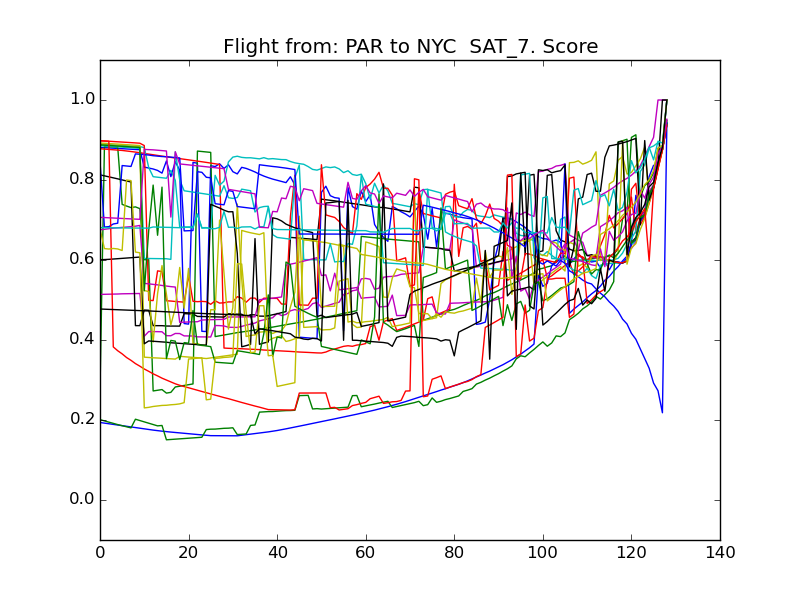
\includegraphics[width=5cm]{../ScoreUNDERESTIMATE/ScorePARNYC_SAT_7.png}
        %\caption{ the model $\beta$ with an under estimation of $p_{min}$}
      \end{figure}
    \end{column}
  \end{columns}
}


\frame{
  \frametitle{comparaison of the models for the flight PARIS-ROMA }
  Form top to bottom and from left to right : the model $\alpha$ , the model $\beta$ with an exact estimation of $p_{min}$, $\beta$ with an over estimation of $p_{min}$and $\beta$ with an under estimation of $p_{min}$

  \begin{columns}
    \begin{column}{5cm}
      \begin{figure}
        \centering
        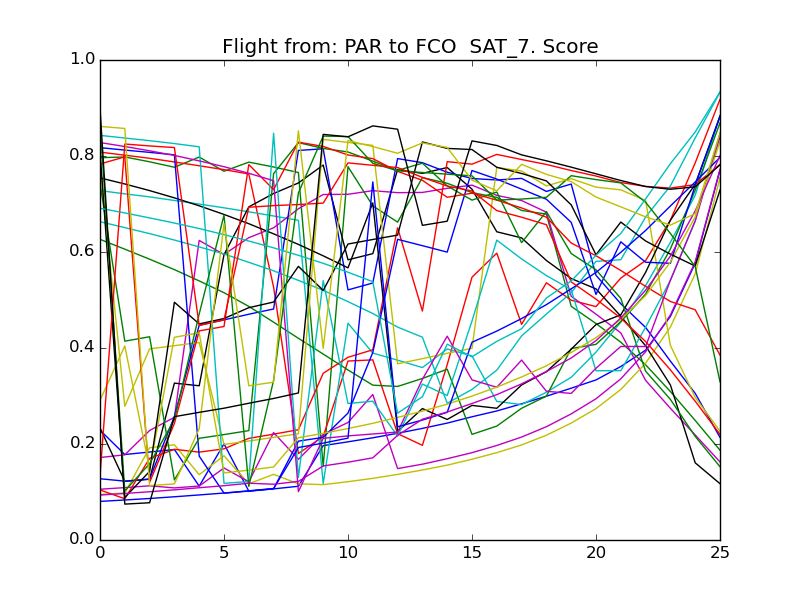
\includegraphics[width=5cm]{../ScoreImg/ScorePARFCO_SAT_7.png}
        %\caption{ the model $\alpha$ }
      \end{figure}

      \vspace{-0.8cm}
      \begin{figure}
        \centering
        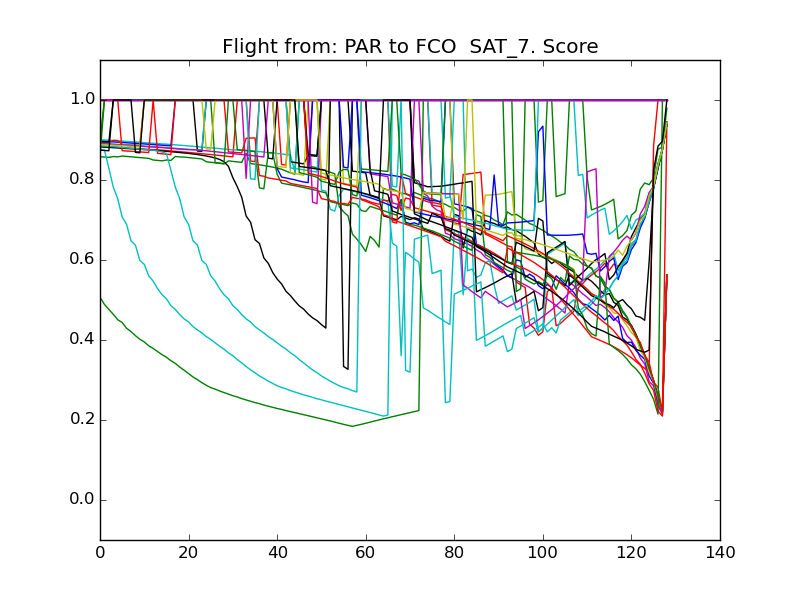
\includegraphics[width=5cm]{../ScorePRECISE/ScorePARFCO_SAT_7.png}
        %\caption{ the model $\beta$ with an exact estimation of $p_{min}$}
      \end{figure}
    \end{column}

    \begin{column}{5cm}
      \begin{figure}
        \centering
        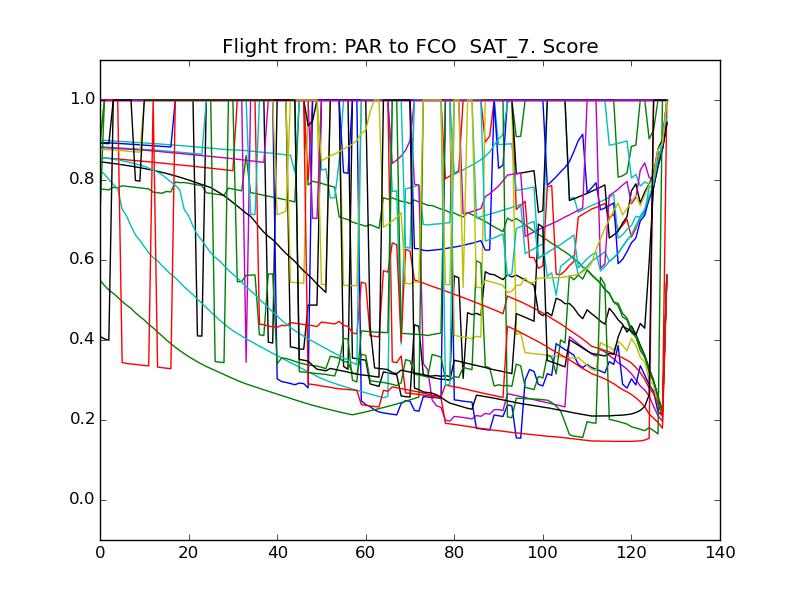
\includegraphics[width=5cm]{../ScoreOVERESTIMATE/ScorePARFCO_SAT_7.png}
        %\caption{ the model $\beta$ with an over estimation of $p_{min}$}
      \end{figure}
      \vspace{-0.8cm}
      \begin{figure}
        \centering
        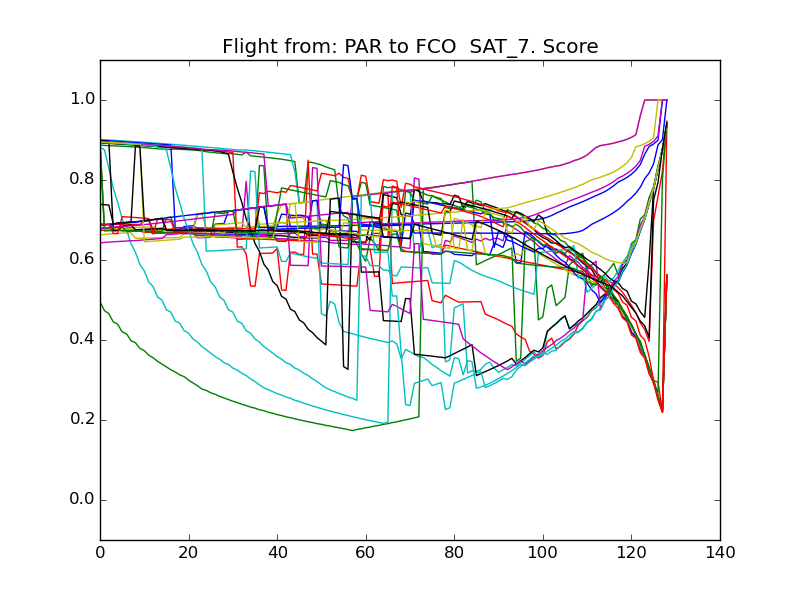
\includegraphics[width=5cm]{../ScoreUNDERESTIMATE/ScorePARFCO_SAT_7.png}
        %\caption{ the model $\beta$ with an under estimation of $p_{min}$}
      \end{figure}
    \end{column}
  \end{columns}
}


\frame{
  Conclusion
  \hspace{0.4cm}
  Primary objective: test algorithms for predicting option success.
  \begin{itemize}
  \item We looked at a score per departure day.
  \item We looked at the average difference between Option Way's
    prediciton and what the data shows.
  \end{itemize}
  Option Way is a very optimistic company.

  \vspace{0.4cm}
  
  Secondary objective: come up with a better prediction.
  \begin{itemize}
  \item The parameters in Option Way's formula can be optimized (on-going).
  \item We propose another model which takes more variable and has
    more parameters.
  \end{itemize}

  \begin{center}
    Thank you for your attention!\\
    Merci pour votre attention!
  \end{center}
}

\end{document}
